\problemname{Grand Central Station}

The city you live in just finished construction of its new transport network,
PlusRail. There are $n$ stations and exactly one way to get between any given
pair of them; this is because there are only $n-1$ direct station:station
connections. In other words, the network forms a tree.

You have been hired to put together the signage for each of the stations which
shows where on the network a passenger is with a big arrow pointing to the
bright red station in the centre.

\begin{figure}[h!]
  \centering
  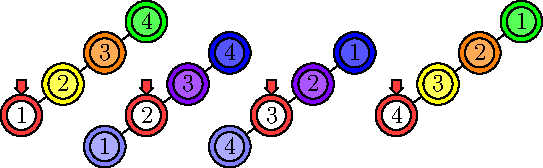
\includegraphics[width=1.0\textwidth]{sample}
  \caption{Illustration of Sample Input 1 and how two designs are reused four
           times, with the labels painted at different places.}
  \label{fig:grandcentral}
\end{figure}

Because the drawings of the network are fairly crude, it is actually possible
that you could use the same sign in more than one station, and just write a
different permutation of labels for the station names.

If you want to make signage for the whole network, what is the minimum number
of unique designs you will need?

\section*{Input}
\begin{itemize}
\item The first line of input contains the number of stations, $n$
      ($1 \le n \le 3 \times 10^5$).

\item The following $n-1$ lines each contain two distinct vertex indices
      $a$ and $b$ ($1 \le a, b \le n$) indicating that there is a direct
      route between these stations.
\end{itemize}

\section*{Output}

Output the minimum number of map designs that can be made, such that for any
station at least one of these map designs can be re-labelled such that this
station is in the centre.
